% This must be in the first 5 lines to tell arXiv to use pdfLaTeX, which is strongly recommended.
\pdfoutput=1
% In particular, the hyperref package requires pdfLaTeX in order to break URLs across lines.

\documentclass[11pt]{article}

% Remove the "review" option to generate the final version.
\usepackage{acl}

\usepackage{graphicx}

% Standard package includes
\usepackage{times}
\usepackage{latexsym}

% For proper rendering and hyphenation of words containing Latin characters (including in bib files)
\usepackage[T1]{fontenc}

% This assumes your files are encoded as UTF8
\usepackage[utf8]{inputenc}

% This is not strictly necessary, and may be commented out,
% but it will improve the layout of the manuscript,
% and will typically save some space.
\usepackage{microtype}

\title{Proposal: Neuro-Symbolism for Feature Importance Explainability of Deep Reinforcement Learning Models}

\author{Roel Leenders \\
  University of Twente, Enschede, The Netherlands \\
  \texttt{r.leenders@student.utwente.nl}} 
\begin{document}
\maketitle
% ENVIRONMENTS: https://agents.inf.ed.ac.uk/blog/multiagent-learning-environments/
% Keywords: knowledge graph completion (KGC),
\section{Introduction}
% ----------------------------------------
% The introduction gives the context of the work and also the motivation for research in this area. Meant 
% is the „external‟ motivation: what is the relevance of this subject.
% ----------------------------------------

% <something about why XAI is important>
% ----------------------------------------

In recent years the field of Artificial Intelligence (AI) has seen an increasing need for explainability. As models became more 
complex and computationally intensive, a performance-transparency trade-off was introduced \cite{Puiutta2020}. High-performing 
models with complex inner workings come at the cost of transparency; it becomes less clear how they achieve their decisions and 
predictions. 

The necessity for explainable AI (XAI) increases particularly for machine learning methods like Reinforcement Learning (RL)
where an agent learns autonomously with little to no human intervention. Additionally, since people are by and large concerned
about the risks of automated decision-making \cite{Araujo2020}, explainability is also important to improve the public opinion and trust of AI.

% something about knowledge graphs and how they can be used to train and explain AI

\section{Problem Statement}
% ----------------------------------------
% This component describes the problem the paper will focus on. The motivation of its relevance and its 
% relationship with the state of the art in the scientific field should be given, with references to the 
% literature. This leads to a number of clearly formulated research questions (usually 3 to 6). The research  
% questions should be operational: they can be answered by the method you are using. Expected answers 
% can be given.  
% A hierarchy in the research questions (main questions with sub questions) can be suitable. In this case 
% the relationship between the main question and the sub questions should be clear. 
% Preferably the research questions are emphasized in lay-out. 
% An important aspect of this component is that it should make clear what the paper contributes to the 
% topic: what is new, what does the research add to the existing knowledge. 
% ----------------------------------------
% <Motivation of the relevance of the paper>
Fortunately, XAI has seen a rapid growth in active research with a plethora of contributions proposing a variety of different techniques \cite{Xu2015, Ribeiro_Singh_Guestrin_2018, ijcai2019-876}. 
Although still understudied, RL has seen emerging XAI trends \cite{Wells2021} which include visualization, query-based explanations and policy summarization. 

An XAI method that makes models inherently more transparent is the use of a knowledge-driven (symbolic) methods \cite{tiddi_knowledge_2022}. Oltramari et al. (\citeyear{Oltramari2020}) propose a method in which
knowledge-driven methods (e.g. knowledge-graphs) can be used in hybrid fashion with deep neural networks. The authors show that this neuro-symbolic approach is able to maintain interpretability while achieving comparable
performance. However, although knowledge-driven methods for XAI are more common within the supervised learning literature \cite{tiddi_knowledge_2022}, knowledge-driven XAI used for RL is still very much understudied.
Therefore, the proposed research focuses on the use of neuro-symbolism to both train and explain the behavior of a RL agent. This results in the following research question and sub-questions:

% <Problem: Currently deep reinforcement learning models are difficult to explain. Knowledge Graphs are an option for better XAI.
% They, however, have not fully been researched for reinforcement learning models>
% <Research Question 1: To what extent, if any, can a domain specific knowledge-graph improve the explainability of a deep RL model?>
% <Sub Question 1: How can a deep RL model use a domain specific knowledge graph?>

\begin{itemize}
  \item \textbf{RQ. 1}: To what extend, if any, can neuro-symbolism improve the feature importance explainability of a deep RL model?
  \item \textbf{SQ. 1}: What are suitable neuro-symbolic architectures for Deep RL models?
  \item \textbf{SQ. 2}: How to evaluate the feature importance explainability of neuro-symbolic architectures of Deep RL models?
\end{itemize}



\section{Proposed Method of Research}
% ----------------------------------------
% This component describes the methodology you are going to use to answer the research questions and 
% motivates why it is suitable. 
% A remark such as „I will perform a literature study to find answers to the questions‟ is too vague. What 
% type of literature, how do you think the literature will lead you to the answers, etc, are all relevant 
% issues. If your methodology involves experiments, you should show how you intend to set up the 
% experiment, how you think the experiment will answer your questions, etc. 
% ----------------------------------------

\begin{figure}[ht]
  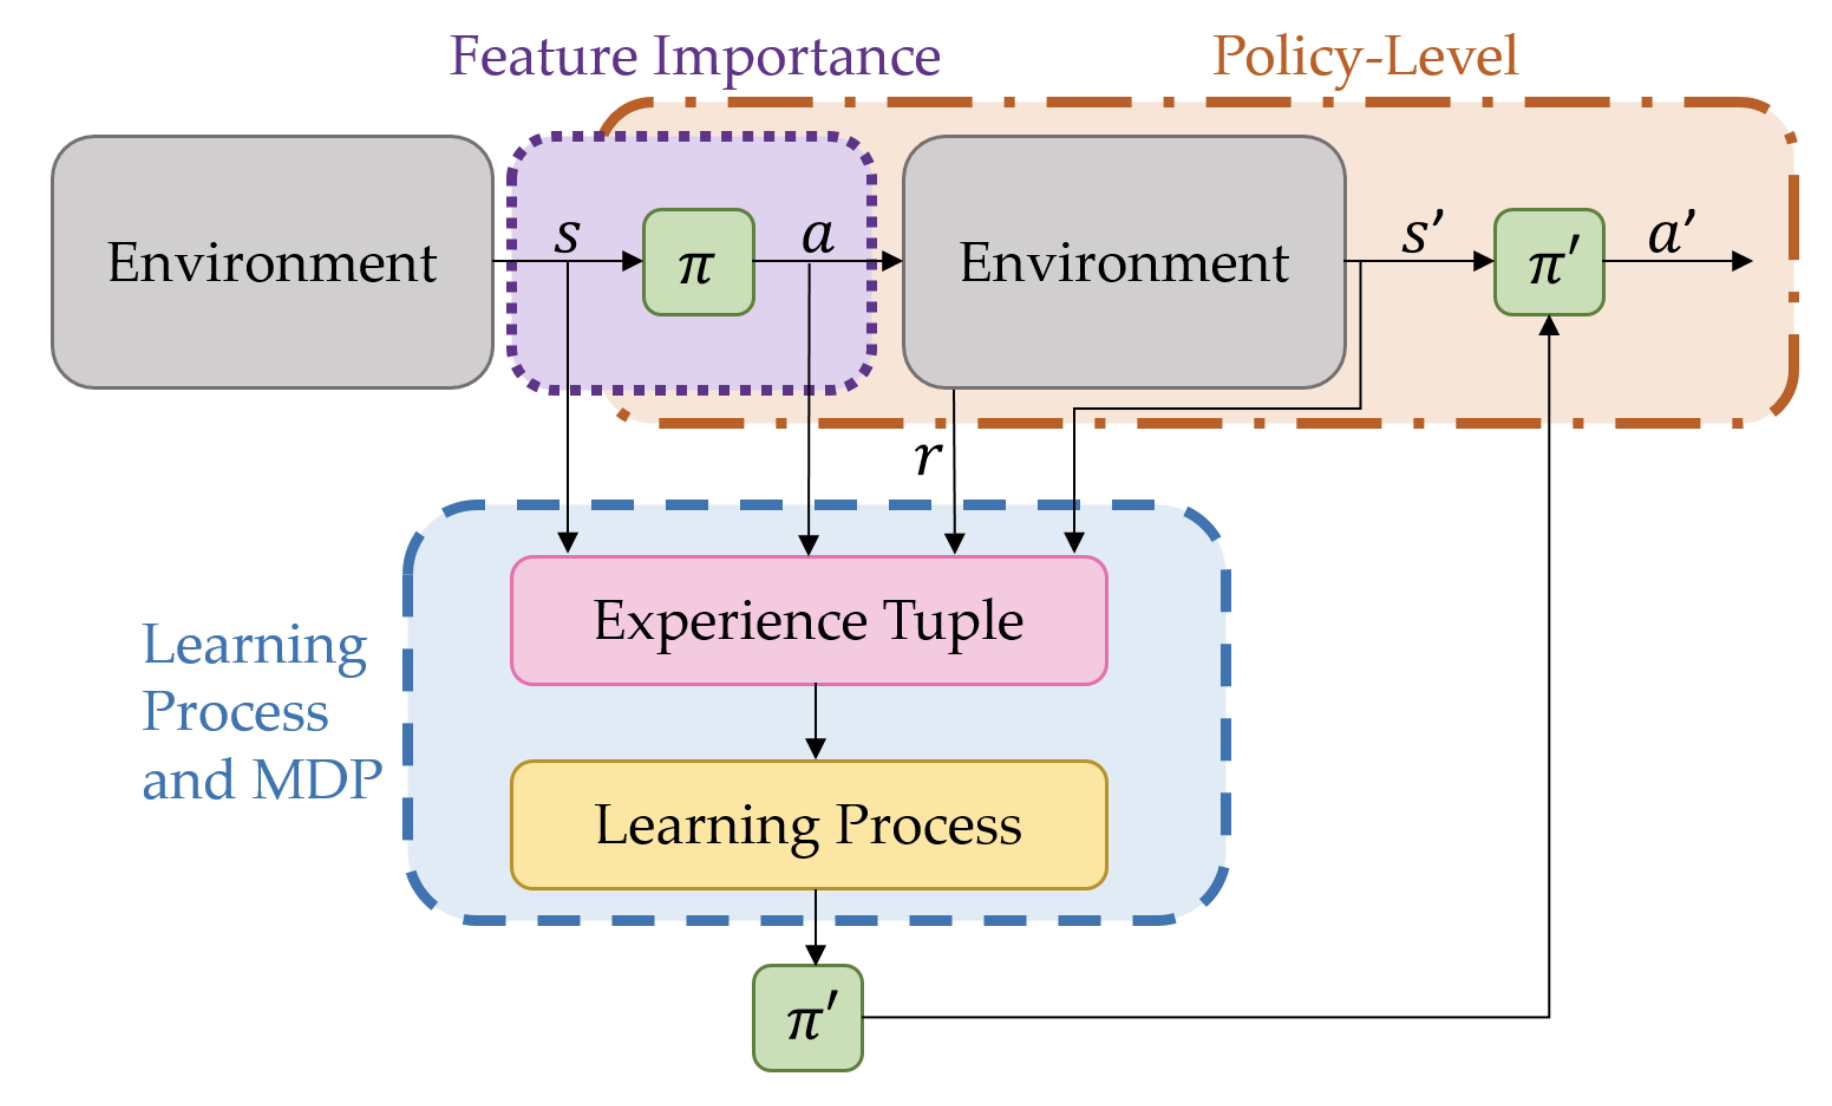
\includegraphics[width=\linewidth]{images/rl_taxonomy.png}
  \caption{RL taxonomy proposed by Milani et al. (\citeyear{Milani2022}) which distinguishes between \textit{feature importance}, \textit{learning process and MDP}, and \textit{policy-level} XAI literature.}
  \label{fig:rl_taxonomy}
\end{figure}

To narrow down the scope of the proposed research, the focus will mainly be on the \textit{feature importance} explainability of a RL model \cite{Milani2022}.
Milani et al. propose a taxonomy for organizing the XAI literature that focuses on RL. This taxonomy distinguishes between three different aspects of explainable RL (see figure \ref{fig:rl_taxonomy}).
In particular, \textit{feature importance} aims to explain the features that affect an agent's decision-making for a given input state.
Most \textit{feature importance} techniques mentioned in the taxonomy use XAI methods extended from supervised learning literature \cite{greydanus_visualizing_2018,goel_unsupervised_2018,ehsan_rationalization_2017}. 
Since there is supporting literature for knowledge-driven XAI in supervised learning, the proposed research will therefore aim to use neuro-symbolism for \textit{feature importance} explainability in deep RL models.

The proposed method of research will consist out of three different phases. First of all, a small literature review will be conducted which aims to provide an overview of the different neuro-symbolic approaches suitable for Deep RL.
Although the literature has already been consulted for this proposal, more in-depth knowledge is required to fully understand how to implement these approaches for both the training and the explaination of Deep RL models.
Additionally, suitable performance and explainability evaluation methods will be explored.

Secondly, a prototype will be built in which a simple RL agent will be trained using the most suitable neuro-symbolic approach. 
In order realise this, a suitable virtual environment has to be chosen for which neuro-symbolism is both applicable and available. 
A suitable option may be the \textit{Monolopy} environment used by Peng et al. (\citeyear{peng_detecting_2021}), which trained a neuro-symbolic RL model that is able to adapt to novelty using a knowledge-graph.

Lastly, the neuro-symbolic model will be evaluated by doing a comparison with a baseline model. In order to perform this comparison a baseline RL model will be trained using a non knowledge-driven method.
During this comparison both the performance and explainability will be evaluated between the different models.

\section{Planning}
% ----------------------------------------
% Mile-stones in terms of concrete content/tasks/products to be delivered should be given. Elements of 
% the schedule should relate to steps in your methodology. E.g., if you need to find something from the 
% literature before you can set up your experiment, write down when you need to have it. Say when you 
% will start the experiment. Say when you will start collecting data. Say how long you will take for 
% analysis. Say when you expect to have the answers to your questions.  
% NB Tasks such as “week 45: research” are NOT concrete enough. 
% ----------------------------------------
The planning for the proposed research can be found in table \ref{tab:planning}

\begin{table}[ht]
  \centering
  \begin{tabular}{|p{0.7cm}|p{6cm}|} 
  \hline
  Week  & Milestone                                                          \\ 
  \hline
  5     & Literature Review: Implementation neuro-symbolic methods for Deep RL     \\ 
  \hline
  6     & Literature Review: Evaluation methods for neuro-symbolic methods   \\ 
  \hline
  6 - 8 & Prototype: Train both neuro-symbolic and baseline models           \\ 
  \hline
  8 - 9 & Evaluation: Compare both models in performance and explainability  \\
  \hline
  \end{tabular}
  \caption{Planning for the proposed research.}
  \label{tab:planning}
  \end{table}
\bibliography{anthology,custom, zotero}

% \appendix

% \section{Example Appendix}
% \label{sec:appendix}

% This is an appendix.

\end{document}
